15.2.3. 例

\begin{enumerate}
\def\labelenumi{(\roman{enumi})}
\item
  当 B 退化为一点时，B 上的 \(C_{K}^{r,s}\) 类流形的概念等价于 \(C^{s}\) 类 K-流形的概念。
\item
  设 Z 是一个 \(C^{s}\) 类 K-流形；取 \(X = B \times Z\) 与 \(p = pr_{1}\)。在 X 上存在、且仅存在一个 B 上的 \(C^{r,s}\) 类流形结构，使得对 Z 的每个卡 \((U, \psi, L)\)，\((B \times U, Id_{B} \times \psi, L)\) 都是 \(C^{r,s}\) -流形 X 的一个卡。
\item
  设 X 是 B 上的一个 \(C^{r,s}\) 类流形，Y 是 X 的一个开子集。由 X 的结构诱导的 Y 的 \(C^{r,s}\) 类流形结构，其定义与流形情形中的做法相同（参见 5.2.3）。
\item
  设 M 是一个以 B 为底、\(C^{r}\) 类的 K 上的向量丛（7.3.4），\(\pi\) 是它到 B 上的投影。在 M 上存在、且仅存在一个 B 上的 \(C_{K}^{r,\omega}\) 类流形结构，使得若 \((\mathbf{U},\psi,\mathbf{F})\) 是 M 的一个 K-向量卡（8.8.1），则三元组 \((\pi^{-1}(\mathbf{U}),\psi,\mathbf{F})\) 是 \(C_{K}^{r,\omega}\) -流形 M 的一个卡。
\end{enumerate}

15.2.4. 设 X 是 B 上的一个 \(C^{r,s}\) 类流形，p 是其投影，L 是一个 K-Banach 空间，f 是 X 到 L 中的一个映射。我们说 f 是 \(C^{r,s}\) 类的，如果对流形 X 的每个卡 (V, \(\psi\) , F)（这里 X 视为 \(C^{r,s}\) -流形），映射 ( \(f|V) \circ \psi^{-1}\) （从 \(\psi(V)\) 到 L 中）是 \(C^{r,s}\) 类的（15.1.6）。这样的映射是 \(C^{r}\) 类的，并且它在 \(X_{b}\) （\(b \in B\)）上的限制是 \(C^{s}\) 类的。

15.2.5. 设 \(g: \mathbf{B} \to \mathbf{B}'\) 是 \(\mathbf{C}^{r}\) 类微分流形的一个态射，并设

\pandocbounded{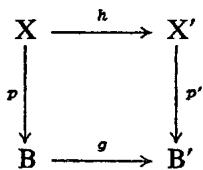
\includegraphics[keepaspectratio]{images/part001_9e08a31f.jpg}}

X（相应地，X'）是 B（相应地，B'）上的一个 \(C^{r,s}\) 类流形，h 是 X 到 X' 中的一个映射。我们说 h 是一个 \(C^{r,s}\) 类 g-态射，如果下列三个条件得到满足：

\begin{enumerate}
\def\labelenumi{\alph{enumi})}
\item
  \(p^{\prime}\circ h = g\circ p;\)
\item
  h 连续；
\item
  对每个卡 \((\mathrm{V}^{\prime},\psi^{\prime},\mathrm{F}^{\prime})\) （\(C^{r,s}\) -流形 \(X^{\prime}\) 的卡），映射 \(pr_{2}\circ\psi^{\prime}\circ h\) 从 \(V=h^{-1}(V^{\prime})\) 到 \(F^{\prime}\) 是
\end{enumerate}

\(\mathbf{C}^{r,s}\) 类的（按 15.2.4 的意义），这里开集 V 赋有由 X 诱导的结构（15.2.3, (iii)）。

当 \(\mathbf{B} = \mathbf{B}'\) 且 \(g = \mathrm{Id}_{\mathbf{B}}\) 时，我们也称 \(h\) 为一个 \(\mathbf{C}^{r,s}\) 类 B-态射。

为使一个 \(C^{r,s}\) 类 B-态射是一个 \(C^{r,s}\) 类 B-同构，只需它是一个 \(C^{1}\) 类同构。

设 \(g': B' \to B''\) 是 \(C^r\) 类流形的一个态射，并设 \(X''\) 是一个 \(C^{r,s}\) 类流形，其底为 \(B''\) 。若 \(h: X \to X'\) 是一个 \(g\) -态射且为 \(C^{r,s}\) 类，而 \(h': X' \to X''\) 是一个 \(g'\) -态射且为 \(C^{r,s}\) 类，则 \(h' \circ h\) 是一个 \((g' \circ g)\) -态射且为 \(C^{r,s}\) 类。

15.2.6. 设 X 是 B 上的一个 \(\mathbf{C}_{\mathbf{R}}^{r,s}\) 类流形，\(p\) 是其投影；我们假设 \(s \neq \omega\) ，X 是分离的，且 \(p\) 是逆紧的（TG, I, § 10, no. 1）。于是，对每个 \(b \in \mathbf{B}\) ，存在 \(b\) 的一个开邻域 U 以及一个 \(\mathbf{C}^{r,s}\) -同构（从 \(p^{-1}(\mathbf{U})\) 到 \(\mathbf{U} \times \mathbf{X}_b\) 上），其中 \(\mathbf{X}_b = p^{-1}(b)\) 。

15.2.7. 设 X 是 B 上的一个 \(C_{K}^{r,s}\) 类流形，p 是其投影，\(\sigma: B \to X\) 是一个 \(C^{r}\) 类截面。我们称一个 \(C_{K}^{r,s}\) 类管状邻域（\(\sigma\) 的）为如下的三元组 (M, N, \(\varphi\) )：其中 M 是一个以 B 为底、\(C^{r}\) 类的 K-向量丛，N 是 \(\sigma(\mathbf{B})\) 在 X 中的一个开邻域，而 \(\varphi\) 是一个 \(C_{K}^{r,s}\) 类 B-同构（从 N 到 M 的一个开子集上，参见 15.2.3 (iv)），它把截面 \(\sigma\) 映为 M 的零截面。

假设 \(s \geqslant r + 1\) ，并且流形 B 是仿紧的、具有 \(\mathbf{C}^{r}\) 类单位分解（5.3.6）；则存在 \(\mathbf{C}_{\mathbb{K}}^{r,s}\) 类管状邻域（\(\sigma\) 的）。

\subsection{截面簇与映射簇}

15.3.1（“截面空间上的 Banach 空间结构”）。设 B 是一个 \(C^{r}\) 类紧微分流形；设 M 是一个以 B 为底、\(C^{r}\) 类的 K 上的向量丛（7.3.4）；用 \(M_{r}\) 表示 M 的底层 \(C^{r}\) 类微分流形，并用 \(\mathcal{S}_{\mathrm{M}}^{\tau}(\mathrm{B})\) 表示 M 的 \(C^{r}\) 类截面所成的 K-向量空间（7.4.1）。在 \(\mathcal{S}_{\mathrm{M}}^{\tau}(\mathrm{B})\) 上，由 \(C^{r}\) -一致收敛拓扑（在 \(\mathcal{C}^{\tau}(\mathrm{B};\mathrm{M}_{r})\) 上，12.3.10）诱导的拓扑使 \(\mathcal{S}_{\mathrm{M}}^{\tau}(\mathrm{B})\) 成为一个 K-Banach 空间。

设 \((\mathrm{U}_{i})_{i\in\mathbb{I}}\) 是 B 的一个有限开覆盖，并且对每个 \(i\in I\) ，设 \(c_{i}=(\mathrm{U}_{i},\varphi_{i},\mathrm{E}_{i})\) 是 B 的一个卡，\(t_{i}=(\mathrm{U}_{i},\psi_{i},\mathrm{F}_{i})\) 是 M 的一个 K-向量卡（8.8.1）。设每个 \(E_{i}\) （相应地，\(F_{i}\) ）都赋有与它在 R（相应地，K）上的 Banach 空间结构相容的范数，并且 \((\mathrm{V}_{i})_{i\in\mathbb{I}}\) 是 B 的一个闭覆盖，使得 \(V_{i}\subset U_{i}\) 对所有 \(i\in I\) 成立。对 \(f\in\mathcal{S}_{\mathrm{M}}^{\tau}(\mathrm{B})\) 与 \(i\in I\) ，用 \(f_{i}\) 表示由 \(\varphi_{i}(\mathrm{U}_{i})\) 到 \(F_{i}\) 的映射，它由下述复合得到：

\[
\varphi_ {i} \left(\mathrm{U} _ {i}\right) \xrightarrow {\varphi_ {i} ^ {- 1}} \mathrm{U} _ {i} \xrightarrow {f} \mathrm{M} \left| \mathrm{U} _ {i} \xrightarrow {\psi_ {i}} \mathrm{U} _ {i} \times \mathrm{F} _ {i} \xrightarrow {\operatorname{pr} _ {2}} \mathrm{F} _ {i}. \right.
\]

规定

\[
\| f \| = \operatorname{Sup} _ {i \in I, p \leqslant r, x \in V _ {i}} \| D ^ {p} f _ {i} (\varphi_ {i} (x)) \|.
\]

映射 \(f\mapsto\|f\|\) 是 \(\mathcal{S}_{\mathrm{M}}^{\tau}(\mathrm{B})\) 上的一个范数，它给 \(\mathcal{S}_{\mathrm{M}}^{\tau}(\mathrm{B})\) 一个 K 上的 Banach 空间结构。

若 N 是空间 M 的一个开子集，则集合 \(\mathcal{S}^{\tau}(\mathbf{B};\mathbf{N})\) （由截面 \(f\in\mathcal{S}_{\mathbf{M}}^{\tau}(\mathbf{B})\) 中满足 \(f(\mathbf{B})\subset\mathbf{N}\) 者组成）在 \(\mathcal{S}_{\mathbf{M}}^{\tau}(\mathbf{B})\) 中是开的。

15.3.2. 设 B 是一个 \(C^{r}\) 类紧微分流形，X 是 B 上的一个 \(C_{K}^{r,s}\) 类（ \(s \geqslant r + 1\) ）流形。若 N 是 X 的一个开子集，则用 \(\mathcal{S}^{r}(B; N)\) 表示 B 上的像含于 N 的 \(C^{r}\) 类截面所成的集合。在 \(\mathcal{S}^{r}(B; X)\) 上存在、且仅存在一个 \(C^{s-r}\) 类 K-流形结构，使得对每个截面 \(\sigma \in \mathcal{S}^{r}(B; X)\) 以及每个管状邻域 (M, N, \(\varphi\) )（\(C_{K}^{r,s}\) 类，\(\sigma\) 的，15.2.7），三元组 ( \(\mathcal{S}^{r}(B; N)\) , \(\varphi^{*}\) , \(\mathcal{S}_{M}^{r}(B)\) )——其中 \(\varphi^{*}\) 是映射 \(f \mapsto \varphi \circ f\) ——是 K-流形 \(\mathcal{S}^{r}(B; X)\) 的一个卡。

在下文中，我们给 \(\mathcal{S}^{r}(\mathbf{B};\mathbf{X})\) 赋以这一结构。

15.3.3. 设 X 是一个 \(C^{r}\) 类紧微分流形，Y 是一个 \(C^{s}(s \geqslant r + 1)\) 类 K-流形。设 \(\mathcal{C}^{r}(X; Y)\) 是从 X 到 Y 中的 \(C^{r}\) 类映射所成的集合（换句话说，取值于 Y 的底层 \(C^{r}\) 类流形中，参见 5.13.1 与 5.14.2）。我们给 \(\mathcal{C}^{r}(X; Y)\) 赋以一个 \(C^{s-r}\) 类 K-簇结构，它由与 \(\mathcal{S}^{r}(X; X \times Y)\) 的等同得到（参见 15.2.3, (ii) 与 15.3.2）。称它为从 X 到 Y 中的 \(C^{r}\) 类映射簇。它的拓扑是 \(C^{r}\) -一致收敛拓扑（12.3.10）。

假设 Y 是分离的；则 \(\mathcal{C}^{r}(X;Y)\) 也是分离的。此外，从 X 到 Y 中的 \(C^{r}\) 类浸入（相应地，嵌入、浸没、满射浸没、平展态射、同构）所成的集合是 \(\mathcal{C}^{r}(X;Y)\) 的一个开子集。

设 \(X'\) 是一个 \(C^r\) 类紧微分流形，\(\varphi: X' \to X\) 是 \(C^r\) 类微分流形的一个态射，而 \(\psi: Y \to Y'\) 是 \(C^s\) 类 K-簇的一个态射。映射 \(f \mapsto \psi \circ f \circ \varphi\) 是一个 \(C^{s-r}\) 类态射（从 \(\mathscr{C}^r(X; Y)\) 到 \(\mathscr{C}^r(X'; Y')\) 中）。

15.3.4（“结构弱化”）。保留 15.3.3 的假设与记号。此外，设 \(s' \in \mathbf{N}_{\mathbf{R}}\) 满足 \(r < s' \leqslant s\) ，并设 \(\mathbf{Y}_{s'}\) 是一个 \(\mathbf{C}^{s'}\) 类实流形，它以 \(\mathbf{Y}\) 为底层（5.13 与 5.14.2）。\(\mathbf{C}^{s'-r}\) 类实流形结构（在 \(\mathcal{C}^r(\mathbf{X}; \mathbf{Y}_{s'})\) 上）是 \(\mathbf{C}^{s-r}\) 类 K-流形结构（在 \(\mathcal{C}^r(\mathbf{X}; \mathbf{Y})\) 上）的底层。

15.3.5. 设 X 与 X' 分别是 \(C^{r}\) 类与 \(C^{r'}\) 类的紧微分流形，且 \(r' < r\) ；设 Y 是一个 \(C^{s}\) 类 K-簇，\(s \geqslant r + 1\) 。令 \(t = \operatorname{Inf}(r - r', s - r)\) 。映射 \((f, g) \mapsto g \circ f\) 是一个 \(C^{t}\) 类态射（从 \(\mathcal{C}^{r}(X'; X) \times \mathcal{C}^{r}(X; Y)\) 到 \(\mathcal{C}^{r'}(X'; Y)\) 中）。

15.3.6（“\(\mathcal{C}^r (\mathrm{X};\mathrm{Y})\) 的切空间”）。在 15.3.3 的假设之下，设 \(f\in \mathcal{C}^r (\mathrm{X};\mathrm{Y})\) ，并设 \(\xi\) 是 \(f\) 处切于流形 \(\mathcal{C}^r (\mathrm{X};\mathrm{Y})\) 的一个切向量。若 \(x\in \mathrm{X}\) ，则用 \(\varepsilon_{x}\) 表示映射 \(g\mapsto g(x)\) （从 \(\mathcal{C}^r (\mathrm{X};\mathrm{Y})\) 到 Y 中）；它是一个 \(\mathbf{C}^{s - r}\) 类态射。\(\xi\) 在 \(\mathrm{T}_f(\varepsilon_x)\) 下的像是一个元素 \(\xi_{x}\) ，它属于 \(\mathrm{T}_{f(x)}(\mathrm{Y})\) ；映射 \(x\mapsto \xi_{x}\) 是一个 \(\mathbf{C}^r\) 类提升，即 \(f\) 在 T(Y) 中的提升（参见 8.6.1），并且可以把它与一个 \(\mathbf{C}^r\) 类截面（属于以 X 为底的向量丛 \(f^{*}\mathrm{T}(\mathrm{Y})\)）等同起来。这样，就得到了切空间 \(\mathrm{T}_f(\mathcal{C}^r (\mathrm{X};\mathrm{Y}))\) 到 Banach 空间 \(\mathcal{S}_{f^{*}\mathrm{T}(\mathrm{Y})}^r (\mathrm{X})\) 上的一个同构。

15.3.7（“\(\mathcal{C}^{p}(\mathrm{X};\mathcal{C}^{q}(\mathrm{Y};\mathrm{Z}))\) 的解释”）。设 X 与 Y 分别是 \(\mathbf{C}^{p}\) 类与 \(\mathbf{C}^{q}\) 类的紧微分流形（ \(1\leqslant p\leqslant+\infty,1\leqslant q<+\infty\) ），并设 Z 是一个 \(\mathbf{C}^{s}\) 类 K-簇，\(s\geqslant p+q\) 。设 \(f\colon\mathrm{X}\times\mathrm{Y}\to\mathrm{Z}\) 是一个连续映射；

对每个 \(x \in X\) ，用 \(f_x\) 表示从 Y 到 Z 的映射 \(y \mapsto f(x, y)\) 。下列两个性质等价：

\begin{enumerate}
\def\labelenumi{\alph{enumi})}
\item
  对任意卡 \(c = (\mathrm{U}, \varphi, \mathrm{E})\) （\(\mathbf{X}\) 的）、任意卡 \(d = (\mathrm{V}, \psi, \mathrm{F})\) （\(\mathbf{Y}\) 的）与任意卡 \(e = (\mathrm{W}, \theta, \mathrm{G})\) （\(\mathbf{Z}\) 的），只要 \(f(\mathrm{U} \times \mathrm{V}) \subset \mathrm{W}\) ，偏导数 \(\mathrm{D}_{\mathbb{E}}^{p'} \mathrm{D}_{\mathbb{F}}^{q'} f'\) （其中 \(f'\) 是 \(f\) 在卡 \(c \times d\) 与 \(e\) 中的表达式，5.3.2）对 \(p' \leqslant p\) 与 \(q' \leqslant q\) 都存在且连续。
\item
  对每个 \(x \in X\) ，映射 \(f_{x}\) 是 \(C^{q}\) 类的，且映射 \(x \mapsto f_{x}\) 是一个 \(C^{p}\) 类态射（从 X 到簇 \(\mathcal{C}^{q}(Y; Z)\) 中）。
\end{enumerate}

\pandocbounded{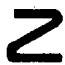
\includegraphics[keepaspectratio]{images/part001_50717dae.jpg}}

15.3.8. 设 Y 是一个 \(C^{s}\) 类紧 K-簇，\(s \geqslant r + 1\) ，并设 \(\text{Diff}^{r}(Y)\) 是 Y 的底层 \(C^{r}\) 类实流形 \(Y_{r}\) 的 \(C^{r}\) 类自同构所成的群。集合 \(\text{Diff}^{r}(Y)\) 在 \(\mathcal{C}^{r}(Y; Y) = \mathcal{C}^{r}(Y_{r}; Y)\) 中是开的；我们给它赋以一个 \(C^{s-r}\) 类 K-簇结构（由 \(\mathcal{C}^{r}(Y; Y)\) 诱导）。复合律 \((f, g) \mapsto g \circ f\) 使 \(\text{Diff}^{r}(Y)\) 成为一个拓扑群。另一方面，\(C^{s-r}\) 类流形结构一般说来与 \(\text{Diff}^{r}(Y)\) 的群结构不相容。对 \(f \in \text{Diff}^{r}(Y)\) ，映射 \(g \mapsto g \circ f\) （从 \(\text{Diff}^{r}(Y)\) 到其自身）是 \(C^{s-r}\) 类的，但映射 \(g \mapsto f \circ g\) 一般说来不是 \(C^{1}\) 类的。特别地，\(\text{Diff}^{r}(Y)\) 一般说来不是一个李群。\footnote{假设 \(s = \infty\)。设 \(\text{Diff}^{\infty}(Y)\) 是 Y 的 \(C^{\infty}\) 类自同构所成的群；给它赋以使诸典范单射 \(\text{Diff}^{\infty}(Y) \to \text{Diff}^{r}(Y)\)（对每个整数 \(r \geqslant 1\)）都连续的最粗拓扑。另一方面，设 \(\text{Diff}^{0}(Y)\) 是 Y 的同胚所成的群，赋以一致收敛拓扑（TG, X, § 3, no. 5, 命题 11）。若 \(\dim Y \geqslant 1\)，则不可能找到一个李群 G 以及从 \(\text{Diff}^{\infty}(Y)\) 到 G 和从 G 到 \(\text{Diff}^{0}(Y)\) 的连续同态，使其复合恰为典范单射（参见 LIE, III, § 4, 习题 7）。}

\specialchapter{记号索引}

\(N_{K}\) : 记号与约定 T(X): 8.1.1 \(\zeta_{c}\) : 8.1.1 T(f): 8.1.2 T(X/Y): 8.1.3 \((\partial/\partial u^{i})\) : 8.1.5 T'(X): 8.2.2 df: 8.2.2 \(\langle\xi, df\rangle\) , D \(_{\xi}(f)\) , \(\xi(f)\) : 8.2.3 \(\varphi^{*}\eta\) : 8.2.6 \(\varphi^{*}\omega\) : 8.2.7 与 8.3.1 \(^{k}\Omega^{p}(U; E)\) : 8.3.1 \(\omega|Y\) : 8.3.1 \(\omega\wedge\omega'\) : 8.3.2 \(i(\xi,\omega)\) , \(i(\xi)\omega\) , \(i(\xi).\omega\) : 8.3.2 \(d\omega\) : 8.3.5 GL(E): 8.4.1 \(\theta_{\xi}.f\) : 8.4.2 \([\xi,\eta]\) : 8.5.1 \(i(\psi,\omega)\) , \(i(\psi)\omega\) , \(i(\psi).\omega\) : 8.6.2 F ⊗ C: 8.8.2 T'(X), T''(X): 8.8.3 Alt \(^{p,q}\) (T(X); F): 8.8.4 \(\omega_{p,q}\) : 8.8.4 \(d'\omega\) , \(d''\omega\) : 8.8.5 \(\partial/\partial z^{k}\) , \(\partial/\partial\bar{z}^{k}\) : 8.8.10 \(dz^{\Delta}\) , \(d\bar{z}^{\Delta}\) : 8.8.10 \(\alpha_{+}\) , \(\alpha_{-}\) , \(\Omega\) : 9.1.4 \(\rho\) , \(\Delta\) : 9.1.5 \(X_{p}\) : 9.2.1 T(X,Y): 9.2.8 F': 9.3.7 \(\xi^{p}\) : 9.4.1 \(\Lambda_{p}(x,y)\) : 9.4.2

\(\mu^{\otimes n}, \mu_{\mathrm{U}}^{\otimes n}: 10.1\)

mod(a): 10.1

Jac(f): 10.1.1

mod(\(\omega\))\(_{\mu}\), \(|\omega|\): 10.1.6

\(\xi'\xi''\), \(\xi''\xi': 10.2.1\)

Or(E): 10.2.1

\(\mathrm{Or}_{\mathrm{M}}\): 10.2.2

\(\lambda_{\mathrm{M}} = (\mathrm{Or}_{\mathrm{M}}, \{\pm 1\}, \mathrm{X}, \pi)\): 10.2.2

\(\tilde{\mathbf{X}}\): 10.2.4

\(\xi_1 \otimes \xi_2: 10.2.6\) \(\tilde{\mathbf{R}}_{\mathrm{M}}\): 10.3.1

\(\tilde{\mathbf{R}}_{\mathbf{X}}\): 10.4.1

\(\alpha(\omega), \int_{\mathbf{X}} g \cdot \omega, \int_{\mathbf{A}} \omega: 10.4.3\) \(\omega|_{\mathrm{Y}}: 10.4.3\) \(\partial A: 11.1.2\) 与 11.3.2

\(\mathrm{T}_a^+(\mathrm{A}), \mathrm{T}_a^-(\mathrm{A}): 11.1.4\) \(\omega|_{\partial A}: 11.2.2\) \(u \perp (t_1, \ldots, t_p): 11.4.1\) \(\tilde{\mathbf{R}}_n: 11.4.2\) \(\omega \perp (t_1, \ldots, t_p): 11.4.5\) \(\int_{\pi|_{\mathrm{A}}} \omega, \int_{\pi} \omega: 11.4.6\) \(j_x^k(f): 12.1.2\) \(s(j), b(j): 12.1.2\) \(\mathrm{J}^k(\mathrm{X}, \mathrm{Y}), \mathrm{J}_x^k(\mathrm{X}, \mathrm{Y}), \mathrm{J}^k(\mathrm{X}, \mathrm{Y})_y, \mathrm{J}_x^k(\mathrm{X}, \mathrm{Y})_y: 12.1.2\) \(j' \circ j: 12.1.4\) \(r^{k, k'}(j): 12.1.5\) \(j_x^\infty(f), j_x^\omega(f): 12.1.6\) \(\mathrm{P}_m(\mathrm{E}; \mathrm{F}): 12.2\) \(\Delta^m f(a), \Delta_a^m(f), \Delta_a^m(j): 12.2.1\) \(\mathrm{Q}^k(\mathrm{E}, \mathrm{F}): 12.2.2\) \(\mathrm{T}(j): 12.3.4\) \(j^k(f): 12.3.7\) \(\mathrm{J}^k(f, g): 12.3.9\) \(\mathrm{GL}^k(\mathrm{E}): 12.4.2\) \(\mathrm{R}^k(\mathrm{E}, \mathrm{X}): 12.4.3\) \(\mathrm{P}_x^k(\pi), \mathrm{P}^k(\pi): 12.5.1\) \(\mathrm{P}^k(g): 12.5.3\) \(\mathrm{P}^k(\mathrm{E}): 12.6.1\) \(\mathrm{P}^k(\mathrm{X}): 12.6.2\) \(\mathrm{P}^k(u): 12.6.3\) \(\tau_m(\mathcal{V}), \tau_m(f), \mathrm{P}_m(\mathrm{E}; \mathrm{F}): 12.6.7\) \(\mathrm{TS}^n(\mathrm{E}), \mathrm{TS}(\mathrm{E}), \mathrm{TS}^{(r)}(\mathrm{E}), \mathrm{TS}^{(r)+}(\mathrm{E}): 13.1.1\) \(\gamma_n(x): 13.1.1\) \(\langle f, t\rangle\): 13.1.2, 13.1.3, 13.2.2, 13.6.1

\(\varphi_{*}(t)\) : 13.1.4 \(\mathrm{T}_x^{(r)}(\mathrm{X}), \mathrm{T}_x^{(k)}(\mathrm{X}), \mathrm{T}_x^{(k)+}(\mathrm{X})\) : 13.2.1 \(\varepsilon_x\) : 13.2.1 \(\langle j, t \rangle\) : 13.2.2 \(\mathrm{T}_x^{(r)}(\varphi), \varphi_*\) : 13.2.3, 13.6.1 \(\mathrm{T}^{(k)}(\mathrm{X}), \mathrm{T}^{(k)+}(\mathrm{X})\) : 13.2.5 \((\Delta_{\xi}^{\alpha})_a\) : 13.2.6 \(\mathrm{gr}_k \mathrm{T}_x^{(r)}(\mathrm{X}), \mathrm{gr} \mathrm{T}_x^{(r)}(\mathrm{X})\) : 13.3.1 \(i, i_x, i_X, i_{X,x}\) : 13.3.1 \(i_k\) : 13.3.1 \(\mathrm{gr}(\varphi_x)\) : 13.3.5 \(t_1 \times t_2, t_1 \otimes t_2\) : 13.4.1 \(\mathrm{T}_x^{(n)}(\mathrm{X}_1, \mathrm{X}_2)\) : 13.4.5 \(\Delta_*\) , \(c\) : 13.5.1 \(\mathcal{T}^{(k)}(\mathrm{X})\) : 13.6.1 \(\mathrm{D}^k (\mathrm{E}, \mathrm{F})\) : 14.1.1 \(\mathcal{D}_{\mathrm{U}}^{k,h}(\mathrm{E}, \mathrm{F})\) : 14.1.1 \(\operatorname{ad}(f)\theta\) : 14.1.4 \(\Delta^\alpha\) : 14.1.6 \(\mathrm{D}_{\mathbf{C}}^{k}(\mathrm{E}, \mathrm{F})\) : 14.1.7 \(\mathrm{D}'' \circ \mathrm{D}'\) : 14.1.8 \([\mathrm{D}' , \mathrm{D}'']\) : 14.1.8 \(\mathrm{S}^k (\mathrm{E}, \mathrm{F})\) : 14.2.1 \(\sigma_k (\mathrm{D})\) : 14.2.1 \(\mathrm{Sym}^k (\mathrm{M}; \mathrm{N})\) : 14.2.2 \(\Omega, \tilde{\mathbf{M}}\) : 14.3.1 \(^t\mathbf{D}\) : 14.3.2 \(\Omega_1, \mathbf{G}\) : 14.3.4 \(\Omega^p\) : 14.4.2 \(\operatorname{grad}(f)\) : 14.4.3 \(\mathbf{C}_{\mathbf{R}}^{r,s}\) : 15.1.1 \(\mathbf{C}_{\mathbf{K}}^{r,\omega}\) : 15.1.2 \(\mathbf{C}^{r,s}\) : 15.1.1, 15.1.2, 15.1.6, 15.2.1 \(\mathcal{S}_{\mathbf{M}}^r (\mathbf{B})\) : 15.3.1 \(\mathcal{S}^r (\mathbf{B}; \mathbf{N})\) : 15.3.1 与 15.3.2 \(\mathcal{C}^r (\mathbf{X}; \mathbf{Y})\) : 15.3.3\\
Diff'(Y): 15.3.8

\specialchapter{术语索引}

适配于块的（卡）：11.1.2 向量丛结构的弱化：8.7.1 积分弧、最大积分弧：9.1.3 C-向量图册、复向量图册：8.8.1 闭半空间的边界：11.1.1 块的边界：11.1.2 边界（带边界的流形）：11.1. 注（1） \(\mathbf{C}^{r,s}\) 类 B-态射：15.2.5 射流的靶：12.1.2 B 上 \(\mathbf{C}^{r,s}\) 类流形的卡：15.2.1 C-向量卡、复向量卡：8.8.1 B 上的卡：15.2.1 Cauchy（公式）：11.2.5 点分布场：13.2.5 \(\mathbf{C}^s\) 类点分布场：13.2.5 向量场：8.2.1 复向量场：8.8.2 余向量场：8.2.2 初始场：8.4.5 \(\mathbf{C}^0\) 类（流形、态射）：记号与约定 \(\mathbf{C}^{r,s}\) 类（函数）：15.1.1 与 15.1.2 \(\mathbf{C}^{r,s}\) 类（映射）：15.1.6 与 15.2.4. \(\mathbf{C}^{r,s}\) 类（g-态射）：15.1.6 与 15.2.5 B 上 \(\mathbf{C}^{r,s}\) 类（流形）：15.2.1 测度的典范类：10.1.4 微分算子的类：14.1.1 向量丛的复化：8.8.2 \((p,q)\) 型分量：8.8.4 两个射流的复合：12.1.4 两个微分算子的复合：14.1.8 共轭（截面）：8.8.2 ≥k 阶接触：12.1.1 无限阶接触：12.1.6 反变（函子）：8.2.7

点分布的余积：13.5.1 积分曲线：9.1.1 与 9.1.7 括号：8.5.1 \(\mathbf{C}^{r,s}\) -相容的（B 上的卡）：15.2.1 \(\mathbf{C}^{r,s}\) -图册：15.2.1 C-向量（丛、卡、图册）：8.8.1 闭半空间：11.1.1 函数的微分：8.2.2 外微分：8.3.5 与 10.3.4 有限支撑集的分布：13.6.1, 13.6.2 有限支撑集的复分布：13.6.2 点分布：13.2.1 阶 ≤k 的点分布：13.2.1 无常数项的分布：13.2.1 叶：9.2.2 连通叶：9.2.2 叶状结构：9.2.2 离散叶状结构、粗叶状结构：9.2.4 诱导叶状结构、逆像：9.2.5 叶化的（卡）：9.2.7 叶状的（流形）：9.2.2 余切丛：8.2.2 C-向量丛：8.8.1 法丛：8.1.3 切丛：8.1.1 纤维的切丛：8.1.3 相对切丛：8.1.3 横截丛：8.1.3 复向量丛：8.8.1 实向量丛：8.8.1 积分流：9.1.2 微分形式：8.3.1 交错微分形式：8.3.1 最大次数的微分形式：10.1.5 全纯（微分形式、向量场）：8.8.9 水平（截面）：9.2.10 奇（微分形式）：10.4.1 诱导（微分形式）：8.3.1 与 11.2.2 可积（向量子丛）：9.3.2 与 9.4.4 可积（微分形式）：10.4.3 局部可积（微分形式）：10.4.3 积分（叶状结构）：9.3.2 积分（子流形）：9.3.1 积分（全微分方程的）：9.3.7 向量子丛的积分：9.3.1

沿纤维的积分：11.4.6 寿命区间：9.1.3 雅可比：10.1.1 射流：12.1.2 无限阶射流：12.1.6 截面的射流：12.5.1 微分形式的模：10.1.6 局部可积模：10.1.5 M-扭曲（微分形式）：10.3.3 M-扭曲（标量丛）：10.3.1 可忽略（局部可忽略集）：10.1.3 Green 算子：14.3.4 复微分算子：14.1.7 有界阶的微分算子：14.1.1 E → F 型、阶 ≤k 的微分算子：14.1.1 多重微分算子：14.1.11 微分算子的阶：14.1.1 可定向（向量丛）：10.2.3 可定向（流形）：10.2.4 由复结构确定的定向：10.2.7 流形的定向：10.2.4 向量丛的定向：10.2.3 态射的定向：10.2.5 定向（定向空间）：10.2.2 偶（微分形式）：10.4.1 块：11.1.2 多面体（部分）：11.3.1 局部多面体（部分）：11.3.1 齐次多项式（映射）：13.1.2 殆复（结构）：8.8.3 定向的乘积：10.2.6 外积：8.3.2 内积：8.3.2 与 8.6.2 B 上 \(\mathbf{C}^{r,s}\) 类流形的投影：15.2.1 正则（点、边界）：11.3.2 提升：8.6.1 内向（向量、严格内向向量）：11.1.4 k 阶标架：12.4.3 切标架：8.1.5 Sard（定理）：10.1.3 标量（微分算子）：14.1.6 标量（多重微分算子）：14.1.11 纤维化的截面：记号与约定 S-态射的 S-定向：11.4.3 外向（向量、严格外向向量）：11.1.4

射流的源：12.1.2

Stokes（公式）：11.2.3 与 11.3.4

微分形式的支撑集：10.4.3

微分算子的符号：14.2.1

切（丛）：8.1.1

与叶状结构相切的（子丛）：9.2.8

点分布的常数项：13.2.1

扭曲（微分形式）：10.4.1

一致 \(C^{k}\) 收敛拓扑：12.3.10

扭曲（标量丛）：10.4.1

微分算子的转置：14.3.2

\((p,q)\) 型（微分形式）：8.8.4

\(\mathbf{C}^r\) 类映射流形：15.3.3

速度：9.1.1

管状邻域：15.2.7

π-扭曲（微分形式）：11.4.2

\(\varphi\)-相关：8.2.6


